\section{Design}
% Metatext
The temporary design is based on the preliminary analysis of sprint 1, and will outline the main features of the design, concerning system structure and components, and the user interface.
\todo{add metatext}

\subsection{System design}
To exploit the availability of sensors on the mobile phone and computational power of the server, the system is developed in two parts: the phone application and an extension of the route system in the \gls{astep} system which handles the analysis and comparison of routes.
The two parts will have their own delegated responsibilities, and will perform the necessary tasks, enabling the system to deliver the service.

% The app
\textbf{The \gls{rs} App}\\
The application, hereafter referenced as the app, is the program executed on a mobile device.
Its responsibilities include the gathering of location data and providing the user interface. 

% device limitations -> app abilities
The task of comparing routes is assumed to require much processing power, and also be able to access location data to get the aforementioned routes.
Performing the route comparisons in the app would require that each user have a copy of every other user's routes.
This is a serious privacy concern as this can enable other applications to leach on to the \gls{astep} system a gather data about when people are home and where they live, and is an aspect we would like to avoid.
As mentioned before, calculating the best route matches would most likely require a lot of processing power, which would drain the battery and produce heat.

Assuming that a central server can handle the analysis of the routes, the application is only required to supply the server with location data.
This is a much better solution as the impact on the battery is reduced, and private information can be contained within the \gls{astep} system.

A service running in the background of the app can handle the location data sampling and transfer to a server.
This service would be kept alive when the application is closed as its own thread, thus being able to record routes even when the app is not in focus on the device.
Because the main objective of the background service is to observe the current activity and transfer the route to \gls{astep}, we call it Observer.
The structure of the class can be seen in Figure \ref{fig:classDiagramSprint1Observer}.
The Observer's main goal is to observe what activity the user is currently performing and receive and push locations accordingly.
There are already implementations for this kind of service in Google Play Services for Android applications and these will be utilized.

\begin{figure}[h]
	\centering
	\begin{tikzpicture}[auto]
	\node[class](Observer){Observer
		\nodepart[align=left, text width=4.1cm]{two}
		-currentActivity : Integer
		\nodepart[align=left, text width=4.1cm]{three}
		+observerActivity() : Integer};
	\node[class, below=of Observer](RouteBuilder){RouteBuilder
		\nodepart[align=left, text width=4.9cm]{two}
		-locations : Location[]\\
		-user : UserInfo
		\nodepart[align=left, text width=4.9cm]{three}
		+RouteBuilder(user : UserInfo)\\
		+addLocation(location : Location)\\
		+buildRoute() : Route};
	\draw[aggregation] (Observer) -- (RouteBuilder);
\end{tikzpicture}
	\caption{The small process which should run at all time to build the routes.}
	\label{fig:classDiagramSprint1Observer}
\end{figure}

The API does also have features for detecting which activity is currently being performed.
This can be used to stop and start the gathering of location data, depending on the given activity.

% The aSTEP core
\textbf{The \gls{astep} Component}\\
On the \gls{astep} server, the route is stored in a database and accessed by the RouteStabilityAnalyser.
This analyzer takes the route and compares it to other routes by the same user, to determine whether this route is a regular occurrence, and hence a stable route.

If the RouteStabilityAnalyser determines that the route is stable, the route should be marked with a tag indicating that the route is stable in the database together with values that indicate when this route is expected to occur next.
The server then uses the RouteSimilarityAnalyser to find matches for the new StableRoute.
The matches are stored and new matches are transmitted to the appropriate devices when possible to inform the users of new matches.

%\begin{figure}[h]
%	\centering
%	\begin{tikzpicture}[auto]
	\node[class](LoginActivity){LoginActivity
		\nodepart[align=left, text width=2.7cm]{two}
			-username : String\\
			-password : String
		\nodepart[align=left, text width=2.7cm]{three}
			+submit()};
	\node[class, below left=1 and -1 of LoginActivity](RegisterActivity){RegisterActivity
		\nodepart[align=left, text width=2.7cm]{two}
			-username : String\\
			-password : String
		\nodepart[align=left, text width=2.7cm]{three}
			+submit()};
	\node[class, below right=1 and -1 of LoginActivity](MainActivity){MainActivity
		\nodepart[align=left, text width=4cm]{two}
			-currentUser : UserInfo
		\nodepart[align=left, text width=4cm]{three}
			+MainActivity(user : UserInfo)\\
			+fetchSuggestedRoutes()};
	\node[interface, right=of MainActivity](ISuggestedRoute){
		\nodepart[align=center, text width=2.8cm]{one}
			<<interface>>\\
			ISuggestedRoute
		\nodepart[align=left, text width=2.8cm]{two}
			-getRoute() : Route};
	\node[class, below=of ISuggestedRoute](SuggestedRoute){SuggestedRoute
		\nodepart[align=left, text width=2.8cm]{two}
			-getRoute() : Route};
		
	\draw[association, dashed] (LoginActivity) -| (MainActivity);
	\draw[association, dashed] (LoginActivity) -| (RegisterActivity);
	\draw[association, dashed] (RegisterActivity) -- (MainActivity);
	\draw[generalization, dashed] (SuggestedRoute) -- node[label] {<<realize>>} (ISuggestedRoute);
	\draw[aggregation](MainActivity)--(ISuggestedRoute);
	
	\node[draw, fit=(MainActivity) (LoginActivity) (RegisterActivity)](PackageBody){};
	\node[draw, above right] at(PackageBody.north west){activities};
\end{tikzpicture}
%	\caption{The class structure of the application.}
%	\label{fig:classDiagramSprint1Application}
%\end{figure}

This is the start of a project that will be further developed upon and expanded in the future, emphasizing the importance of reuse in the server, to reduce the number of specialized server resources.
By isolating parts that are specific to the rideshare app on the server, most of this system would be reusable.
An example of how this is achieved through object-oriented design, is the RouteAnalyser seen in Figure \ref{fig:classDiagramSprint1Server}.
The RouteAnalyzer filter routes according to its concrete implementation.
After the filtering, the RouteAnalyser compare the routes.
This enables other projects to develop their own filters and comparison functions for later projects.

\begin{figure}[h!]
	\centering
	\begin{tikzpicture}[auto]
	\node[class](Route){Route 
		\nodepart[align=left, text width=6.3cm]{two}
			-id : Integer\\
			-user : UserInfo\\
			-points : Location[]
		\nodepart[align=left, text width=6.3cm]{three}
			+Route(user : UserInfo, points : Location[])\\
			+getUser() : UserInfo\\
			+getPoint(index : Integer) : Location};
	\node[class, below=of Route](StableRoute){StableRoute
		\nodepart[align=left, text width=6.3cm]{two}
			-days : WeekDays\\
			-departureTime : Time\\
			-arrivalTime : Time
		\nodepart[align=left, text width=6.7cm]{three}
			+StableRoute(route : Route, days : WeekDays)\\
			+getArrivalTime() : Time\\
			+getDepartureTime() : Time};
	\node[class, below=of StableRoute](RouteStabilityAnalyser){RouteStabilityAnalyser
		\nodepart[align=left, text width=4.6cm]{two}
			-isStable : Boolean\\
			-currentRoute : Route
		\nodepart[align=left, text width=4.6cm]{three}
			+getStableRoute() : StableRoute\\
			+analyse(route : Route)};
	\node[class, right=of StableRoute](RouteAnalyser){\textit{RouteAnalyser}
		\nodepart[align=left, text width=3.4cm]{two}
			-id : Integer
		\nodepart[align=left, text width=3.4cm]{three}
			+analyse(route : Route)};
	\node[class, right=of RouteStabilityAnalyser](RouteSimilarityAnalyser){RouteSimilarityAnalyser
		\nodepart[align=left, text width=3.4cm]{three}
			+analyse(route : Route)};
	\node[interface, below=5 cm of RouteAnalyser](RouteComparer){
		\nodepart[align=center, text width=4cm]{one}
		<<interface>>\\
		IRouteComparer
		\nodepart[align=left, text width=5.9cm]{two}
			+compare(x : Route, y : Route) : Integer};
	\node[class, below=of RouteComparer](TimeDistanceComparer){TimeDistanceComparer
		\nodepart[align=left, text width=5.9cm]{three}
			+compare(x : Route, y : Route) : Integer};
	
	\draw[aggregation,transform canvas={xshift=1.3cm}] (RouteAnalyser) -- (RouteComparer);
	\draw[association, dashed,transform canvas={xshift=-1.3cm}] (RouteStabilityAnalyser) -- node[label]{<<build>>} (StableRoute);
	
	\draw[generalization] (StableRoute) -- (Route);
	\draw[generalization] (RouteStabilityAnalyser.north) -- ++(0,0.5) -| (RouteAnalyser);
	\draw[generalization] (RouteSimilarityAnalyser.north) -| (RouteAnalyser);
	\draw[generalization, dashed] (TimeDistanceComparer) -- node[label]{<<realize>>} (RouteComparer);
	\draw[association] (RouteAnalyser) |- node[label, at end, xshift=0.3cm]{0..*} (Route.east);
\end{tikzpicture}
	\caption{The structure of the system inside the server.}
	\label{fig:classDiagramSprint1Server}
\end{figure}

Because commuters were our target and commutes are most likely to occur on a weekly basis, a weekly stability was decided upon.
This means that the RouteStabilityAnalyser can be limited to analyze only two months of data, as the route can be stopped driven.

\subsection{User Interface Design}
% General Introduction to UI - what + why
The user interface (UI) provides interaction methods between the user and the app.
As the priority of this project is functionality with regards to data collection and route generation and comparison, the UI will not be developed together with users, nor allocated excessive resources. 
The UI is developed for practical purposes, like testing, and to lay the basis for further development, but is still held to some standard which will be documented in the following text. 

\subsubsection{Design language}
% Definition
The design language is the general look and appearance of a system.
This is the foundation for the impressions and feels of the user, and affects the user experience.
The design language is selected in collaboration with another aSTEP project group, SW604F16.

% Goals
The user interface is designed to achieve the following usability characteristics \cite{DIS2014}:
\begin{itemize}
	\item Learnability
	\item Utility
	\item Safety
	\item Effectiveness
\end{itemize}

% Material design
The UI is designed to comply with the Google's Material design guidelines \cite{materialDesign}, being ``\textit{bold, graphic, intentional}''. 
Some of the Material design properties are stated in the following list, compiled of citations from the design guidelines \cite{materialProperties}:

\begin{enumerate}
	\item Material has varying x \& y dimensions (measured in dp) and a uniform thickness (1dp).
	\item Material casts shadows. Shadows result naturally from the relative elevation (z-position) between material elements.
	\item Content is displayed on material, in any shape and color. Content does not add thickness to material.
	\item Input events cannot pass through material.
	\item Material cannot pass through other material. For example, one sheet of material cannot pass through another sheet of material when changing elevation.
	\item Material grows and shrinks only along its plane.
	\item Material never bends or folds.
	\item Material can be spontaneously generated or destroyed anywhere in the environment.
\end{enumerate} 

% Paragraph regarding selection of material
Adhering the material design guidelines makes the app achieve a similar aesthetic and usage method as other apps in the Android eco-system. 
The design language aims to make the interface clean and simple, regarding colors and input methods.

\subsubsection{User interface}
% Actions in UI and design thereof
The design drafts in Figure \ref{fig:GUI-firstrun} reflect the necessary functions and the previously described design language. 

% Login and registering pages design
As the user needs a user profile in the aSTEP system to use the app, the users must be able to login if they already have a user profile, or create a new user profile.

\begin{figure}[h!]
	 \centering
	 \begin{subfigure}[b]{0.3\textwidth}
	 	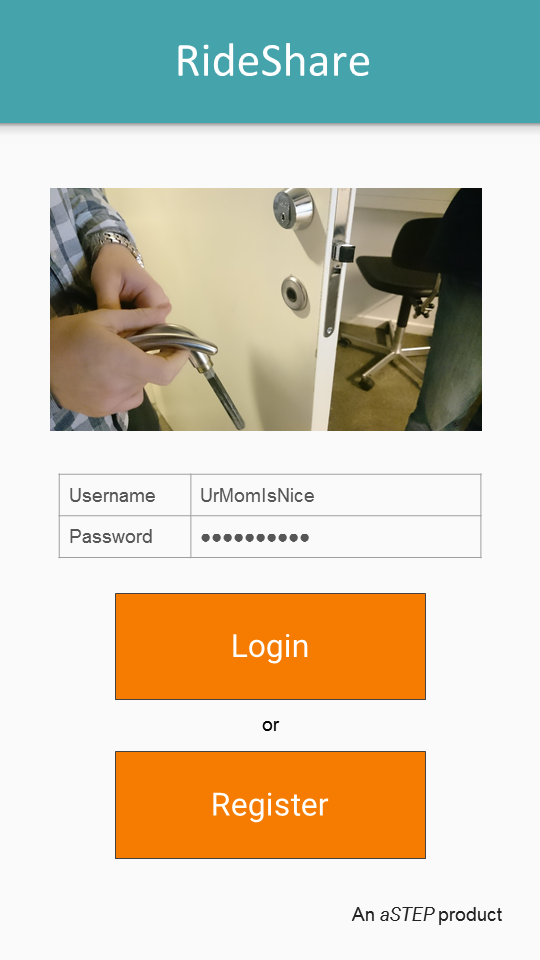
\includegraphics[width=\textwidth]{figures/GUI-front.png}
	 	\caption{Login page}
	 	\label{fig:GUI-front}
	 \end{subfigure}
	 ~ %add desired spacing between images, e. g. ~, \quad, \qquad, \hfill etc. 
	 %(or a blank line to force the subfigure onto a new line)
	 \begin{subfigure}[b]{0.3\textwidth}
	 	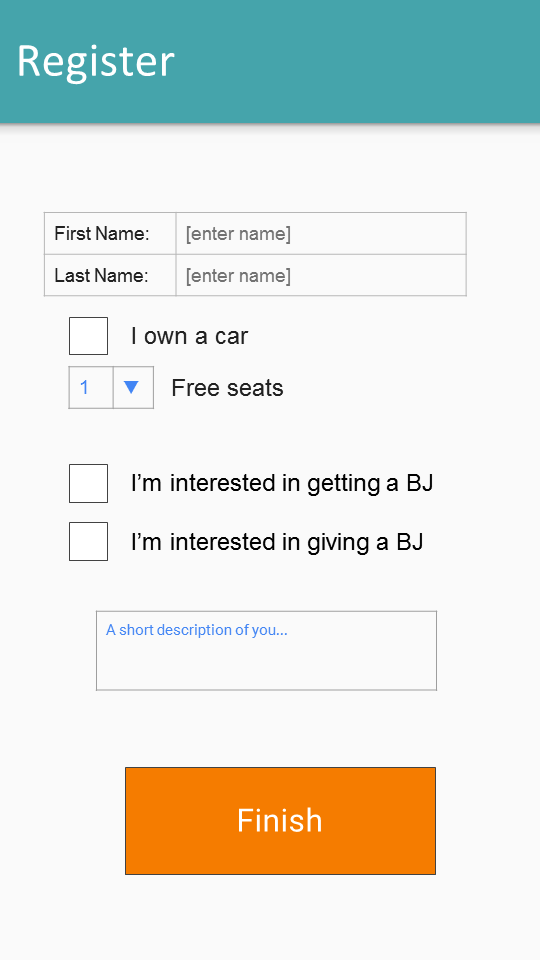
\includegraphics[width=\textwidth]{figures/GUI-register.png}
	 	\caption{Register page}
	 	\label{fig:GUI-register}
	 \end{subfigure}
	 \caption{Draft of the login and registering pages of the app.}\label{fig:GUI-firstrun}
\end{figure}

% In-app pages design
Several screens are necessary to support the different parts of the app. 
The app needs a screen for login, registering, presentation of matches, and a settings page, as can be seen in the figures in Figure \ref{fig:GUI-in-app}.

\begin{figure}[h!]
	\centering
	\begin{subfigure}[b]{0.3\textwidth}
		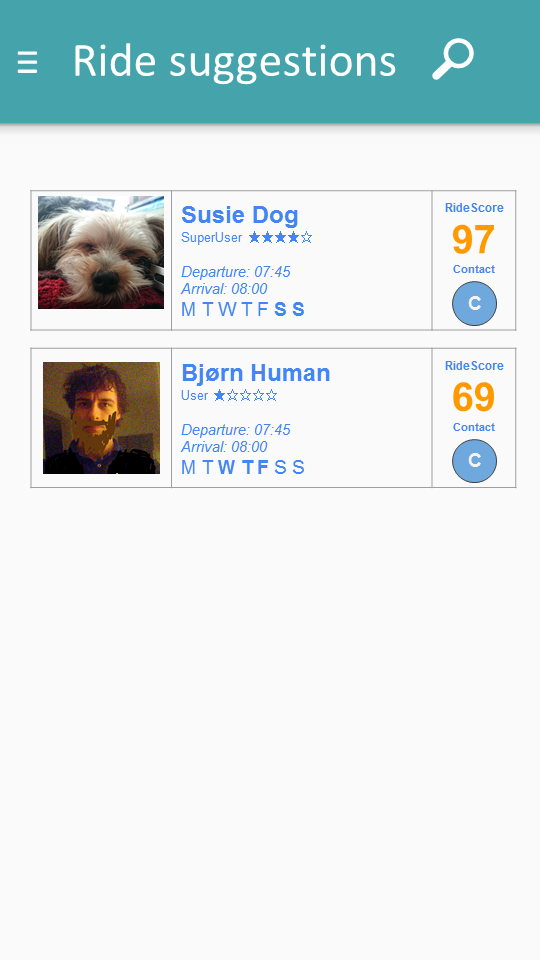
\includegraphics[width=\textwidth]{figures/GUI-main.png}
		\caption{Main page}
		\label{fig:GUI-main}
	\end{subfigure}
	~ %add desired spacing between images, e. g. ~, \quad, \qquad, \hfill etc. 
	%(or a blank line to force the subfigure onto a new line)
	\begin{subfigure}[b]{0.3\textwidth}
		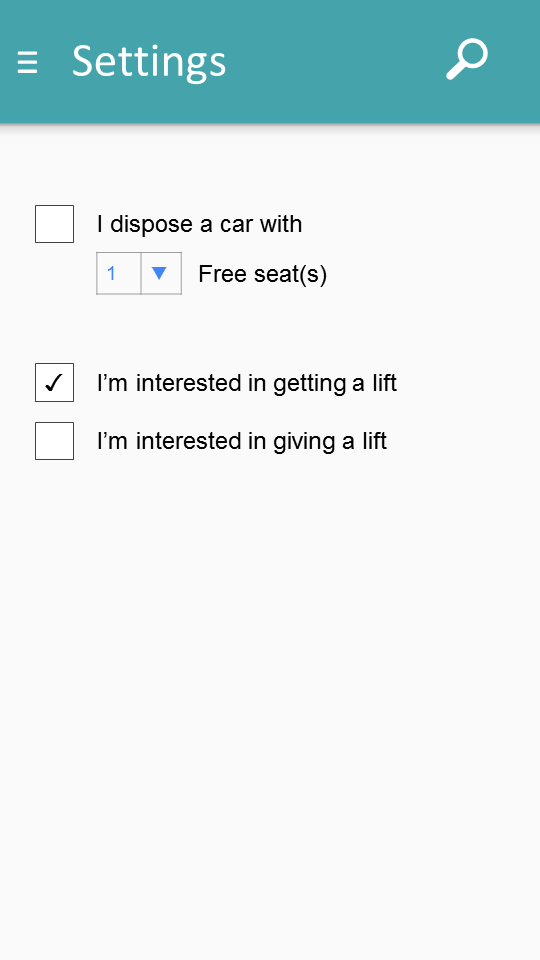
\includegraphics[width=\textwidth]{figures/GUI-settings.png}
		\caption{Settings page}
		\label{fig:GUI-settings}
	\end{subfigure}
	\caption{Draft of the in-app pages of the app.}\label{fig:GUI-in-app}
\end{figure}


